% !TEX program = lualatex
\documentclass[11pt]{article}

% -------- LuaLaTeX : polices et langue --------
\usepackage{fontspec}
\setmainfont{Latin Modern Roman}
\setsansfont{Tex Gyre Heros}
%\renewcommand{\familydefault}{\sfdefault} % force le sans serif par défaut
\usepackage{polyglossia}
\setdefaultlanguage{french}

% -------- Mise en page --------
\usepackage[a4paper,margin=1cm]{geometry}
\usepackage{multicol}
\usepackage{fancyhdr}
\pagestyle{empty}
\usepackage[most]{tcolorbox}

% -------- Mathématiques --------
\usepackage{amsmath,amssymb,mathtools}
\usepackage{icomma}
% \sisetup{locale=FR}

\usepackage{enumitem}
\setlist[itemize]{left=0pt}
\setlist[enumerate]{left=0pt, label=\textbf{\arabic*}.}

\usepackage{ProfCollege}
\usepackage{ProfMaquette}

\usepackage{tabularray}

% -------- Divers --------
\setlength{\parindent}{0pt}

\begin{document}

\begin{multicols}{2}

\begin{Maquette}[Fiche]{Theme=Calcul littéral, Niveau=Troisième}

\begin{exercice}
    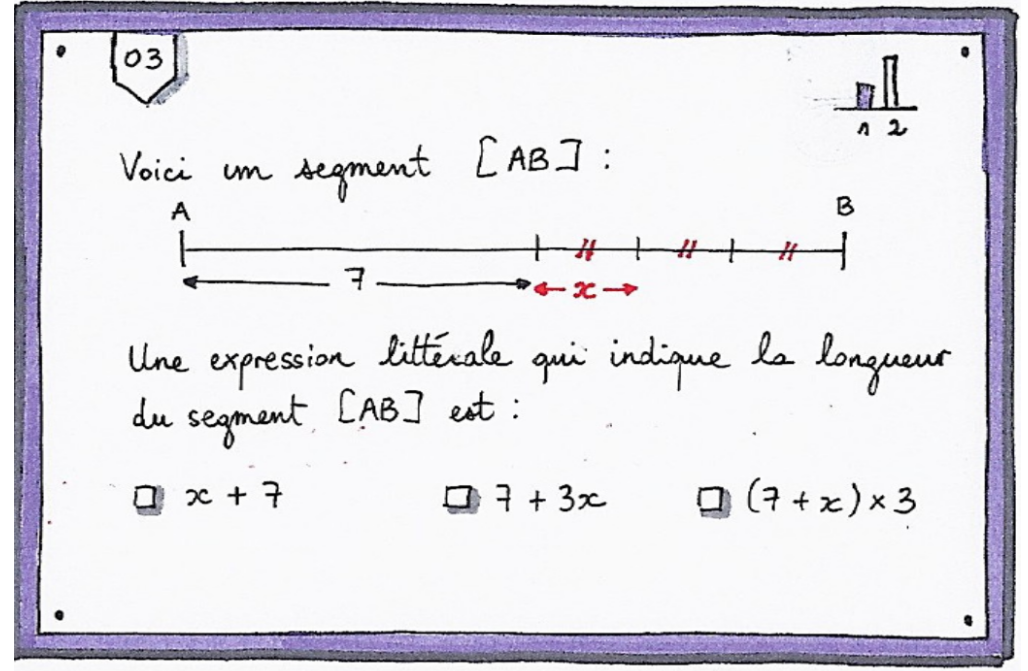
\includegraphics[width=\linewidth]{Images/CalculLitteral1.png}
    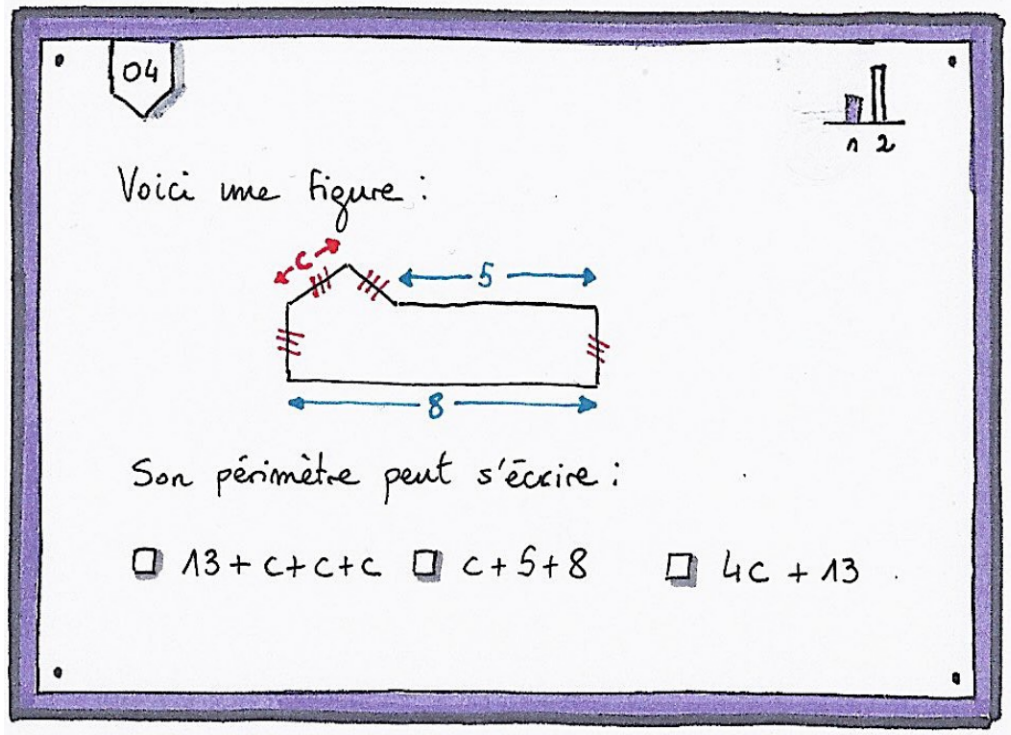
\includegraphics[width=\linewidth]{Images/CalculLitteral2.png}
\end{exercice}

\begin{exercice}
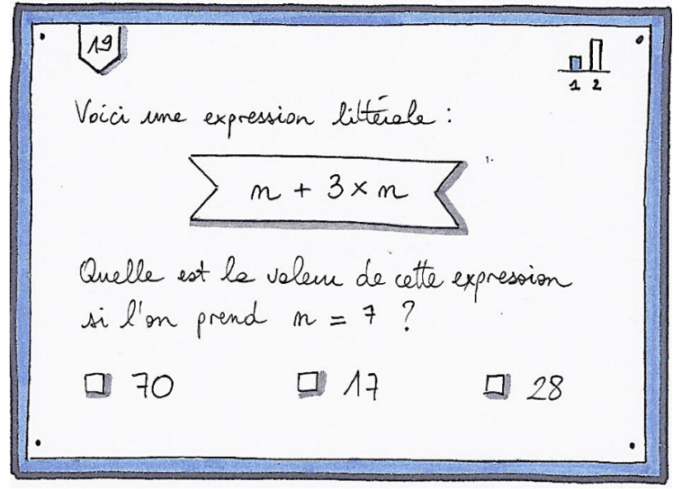
\includegraphics[width=0.95\linewidth]{Images/CalculLitteral3.png}
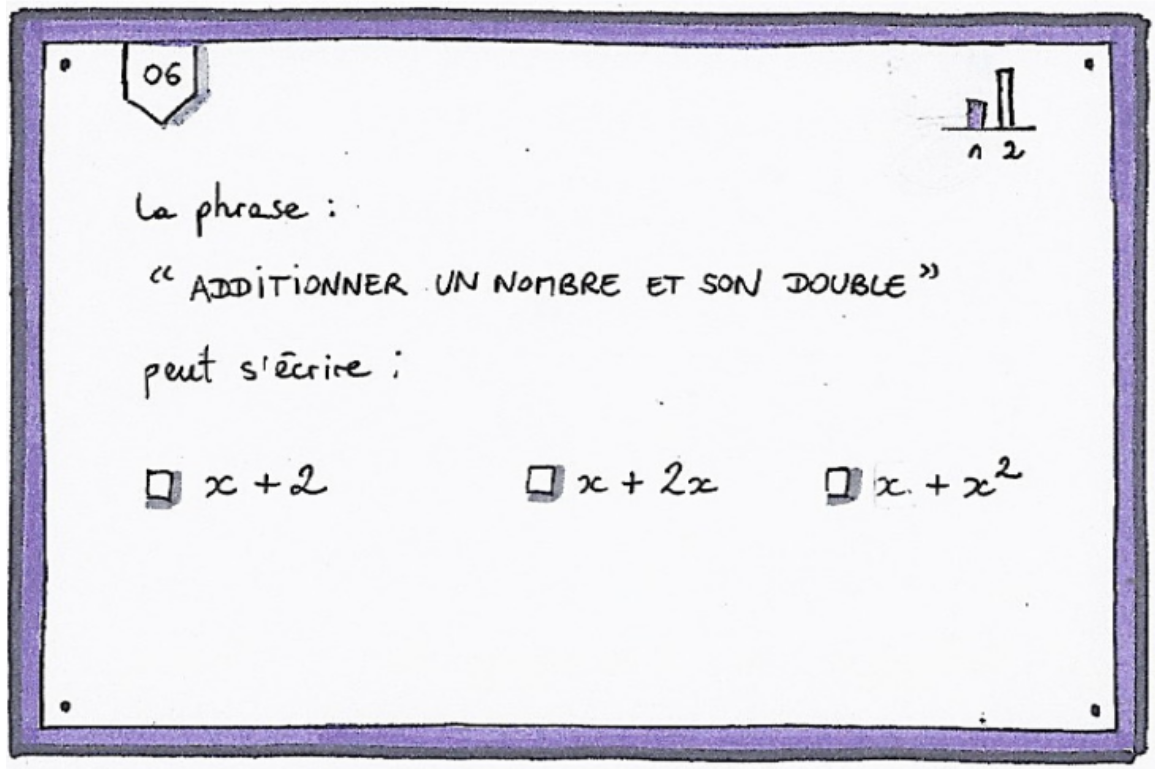
\includegraphics[width=0.95\linewidth]{Images/CalculLitteral4.png}
\end{exercice}

\begin{exercice}
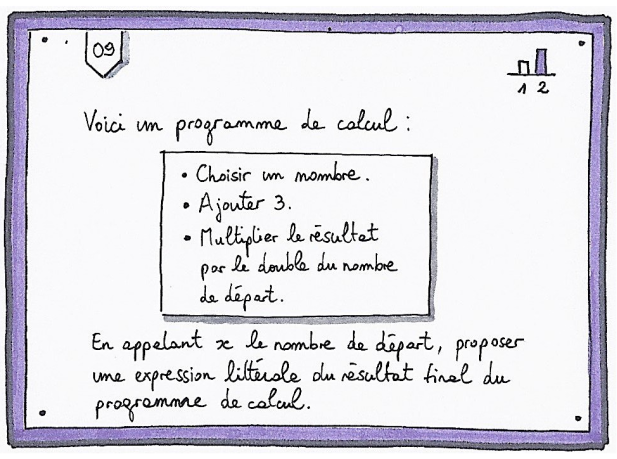
\includegraphics[width=0.95\linewidth]{Images/CalculLitteral5.png}
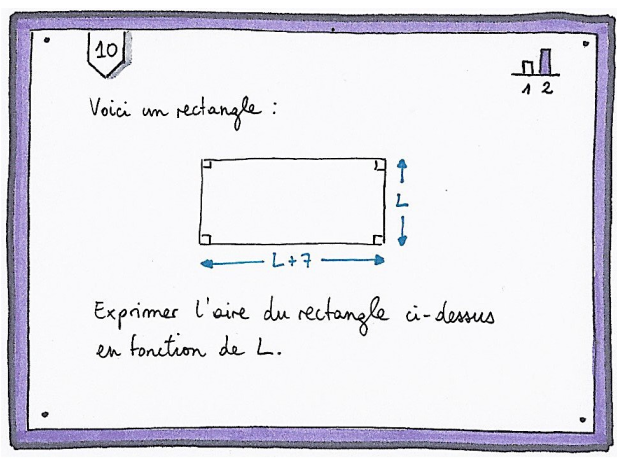
\includegraphics[width=0.95\linewidth]{Images/CalculLitteral6.png}
\end{exercice}

\begin{exercice}
    Réduire les exepressions suivantes.
    \begin{multicols}{2}
        \begin{enumerate}[label=\textbf{\alph*.}]
        \item $6\times x$
        \item $x \times 7$
        \item $6\times a \times 2$
        \item $a \times 3 \times b$
        \item $4\times x \times 10\times y$
        \item $2\times x \times 4 \times x$
        \item $2x\times 5$
        \item $3a \times 2a$
        \item $-3 \times c \times 5$
    \end{enumerate}
    \end{multicols}
\end{exercice}


\begin{exercice}
    Réduire les exepressions suivantes.
    \begin{enumerate}[label=\textbf{\alph*.}]
        \item $6x + 2x$
        \item $6x + 2$
        \item $3a + 2 + 5a$
        \item $20y - 5 -2y$
        \item $5a + 10b - 2a + 3b$
        \item $3x -2 -2x + 10$
        \item $s + 9t + s - 10t$
        \item $5x^2 + 10x - 2x^2 + 4 - x + 1$
    \end{enumerate}
\end{exercice}

\columnbreak


\begin{exercice}
    Réduire les exepressions suivantes.\\
    \emph{Recopier chaque expression, souligner les produits prioritaires, les réduire puis terminer en réduisant les sommes et différences.}
    \begin{enumerate}[label=\textbf{\alph*.}]
        \item $6 + 2 \times x$
        \item $4 \times s + s \times 5 - 3$
        \item $-10 + 3 \times s + 2 \times 2$
        \item $y \times 5 + 3 - 2 \times y$
        \item $3 - 3 \times x + x \times 5$
        \item $4 \times 4 - 4 \times y - 4$
        \item $5 \times 3 + 2 \times d - 4$
        \item $5 + 3 \times e - 2 \times 3$
        \item $3 \times m - 3 \times m + 4$
        \item $8 \times h - 10 - h \times 7$
        \item $3 \times i + 4 \times 2 - i \times 2$
    \end{enumerate}
\end{exercice}

\begin{exercice}
    Recopier chaque expression, supprimer les parenthèses et réduire.\\
    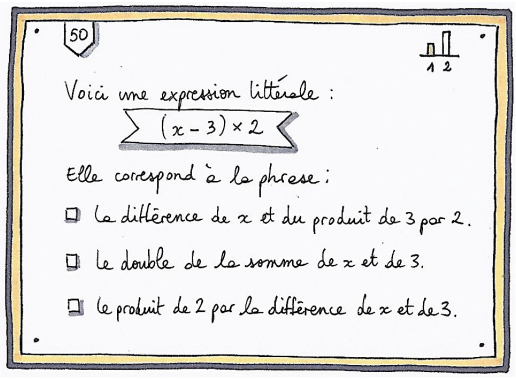
\includegraphics[width=\linewidth]{Images/CalculLitteral7.png}
\end{exercice}

\columnbreak

\begin{exercice}
    Même consigne.\\
    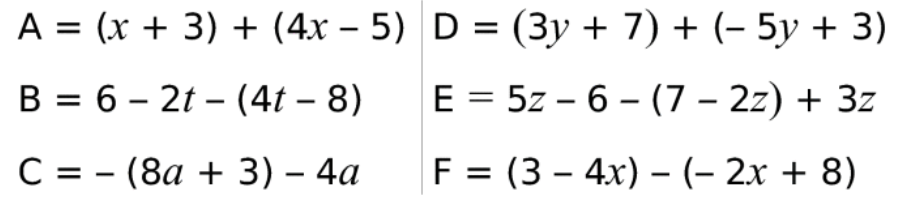
\includegraphics[width=\linewidth]{Images/CalculLitteral8.png}
\end{exercice}


\begin{exercice}
    Recopie chaque pyramide puis détaille sur ton cahier les calculs nécessaires pour compléter les cases vides en respectant les règles indiquées à droite.\\
    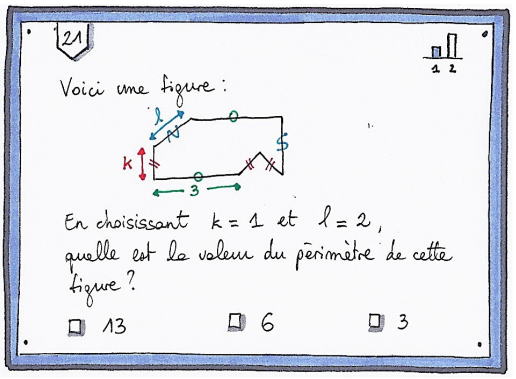
\includegraphics[width=\linewidth]{Images/CalculLitteral9.png}
\end{exercice}


\end{Maquette}

\end{multicols}

\end{document}
 